% Reference (supervisor's Results section), inert. His section is titled
% "Results and Discussions" and folds discussion into the same section as
% subsections rather than a separate top-level section, which is why the
% Discussion content below is nested here as a subsection.
\section{Results and Discussions}
\label{sec:results}

\subsection{A classical model matches a transformer on DAIGT V2 but not on HC3}

\begin{table}[!ht]
\centering
\caption{All eight configurations per corpus. Transformer rows are deployed checkpoints, never grid maxima. Error rate accompanies F1, which saturates here. Bold marks the best classical and best overall F1 per corpus.}
\label{tab:allmodels}
\footnotesize
\setlength{\tabcolsep}{3.5pt}
\begin{tabular}{@{}llcccc@{}}
\toprule
& & \multicolumn{2}{c}{DAIGT V2} & \multicolumn{2}{c}{HC3} \\
\cmidrule(lr){3-4}\cmidrule(lr){5-6}
Model & Rep. & F1 & err\,\% & F1 & err\,\% \\
\midrule
Naive Bayes & BoW & 0.9591 & 4.09 & 0.8713 & 12.87 \\
Naive Bayes & TF-IDF & 0.9577 & 4.23 & 0.8670 & 13.28 \\
Logistic Reg. & BoW & 0.9893 & 1.07 & \textbf{0.9551} & 4.49 \\
Logistic Reg. & TF-IDF & 0.9857 & 1.43 & 0.9365 & 6.35 \\
SVM & BoW & 0.9870 & 1.30 & 0.9475 & 5.25 \\
SVM & TF-IDF & \textbf{0.9910} & 0.90 & 0.9449 & 5.51 \\
BERT & raw & 0.9916 & 0.84 & 0.9916 & 0.84 \\
DeBERTa & raw & \textbf{0.9917} & 0.83 & \textbf{0.9972} & 0.28 \\
\bottomrule
\end{tabular}
\end{table}

Table~\ref{tab:allmodels} reports every configuration on both datasets, and the two benchmarks part company. On DAIGT V2 the best classical configuration, an SVM over TF-IDF at 0.9910 weighted F1, sits 0.0007 below the best transformer, and on the same documents the two disagree on 99 cases split 47 to 52, so McNemar returns $p=0.69$ and the paired interval on the error difference, $[-0.21, +0.34]$ points, contains zero. On HC3 the same comparison is 0.9551 against 0.9972, 484 discordant cases split 16 to 468, $p < 10^{-6}$, and an error difference of $+4.21$ points with interval $[+3.82, +4.61]$, an error-rate ratio of sixteen to one.

\begin{figure*}[!t]
\centering

\includegraphics[width=\textwidth]{figures/fig_roc_zoom.pdf}
\caption{ROC curves for all eight configurations, restricted to the low-false-positive region where the models differ. Areas under the full curve are given in the legend. Each series carries a distinct dash pattern, so the ordering survives greyscale.}
\label{fig:roczoom}
\end{figure*}

Figure~\ref{fig:roczoom} gives the corresponding ROC curves in the region that matters for a deployed detector, where a false positive is an accusation. Over the full range both corpora look alike, every curve close to the corner, and only this view separates them.

Every transformer figure above is the seed-42 checkpoint. Repeating each of the four at seeds 123 and 456 moves them very little. DAIGT V2 BERT averages 0.9921 over a range of 0.0011 and DeBERTa 0.9930 over 0.0024, so the two overlap and the tie is not a seed accident. HC3 BERT averages 0.9930 over 0.0036 and DeBERTa 0.9970 over 0.0005, and those two ranges are disjoint, so the separation that matters to this paper survives reseeding while the tie that also matters survives it in the other direction.

Ranking by area does not reproduce ranking by F1. BERT takes the higher area on DAIGT V2, 0.999641 against 0.999144, while DeBERTa takes the higher F1, and neither ordering survives contact with the predictions, which disagree on 75 documents split 37 to 38 at $p=1.00$. On HC3 the pair separates cleanly. We report both measures because of this, and read neither ordering on DAIGT V2 as a result.

\subsection{The DAIGT V2 tie is a text budget, not an architecture result}
\label{sec:budget}

\begin{table}[!ht]
\centering
\caption{Classical models refitted on the exact character span each transformer's tokeniser kept, so both sides read the same text. The window comes from offset mapping, with no decode round-trip.}
\label{tab:budget}
\footnotesize
\setlength{\tabcolsep}{3.5pt}
\begin{tabular}{@{}llcccc@{}}
\toprule
& & chars & \multicolumn{2}{c}{best classical err\,\%} & transf. \\
\cmidrule(lr){4-5}
Data & Window & kept & full text & 128-tok & err\,\% \\
\midrule
DAIGT V2 & BERT & 0.335 & 0.90 & 2.10 & 0.84 \\
DAIGT V2 & DeBERTa & 0.341 & 0.90 & 2.09 & 0.83 \\
HC3 & BERT & 0.746 & 4.49 & 5.66 & 0.84 \\
HC3 & DeBERTa & 0.756 & 4.49 & 5.72 & 0.28 \\
\bottomrule
\end{tabular}
\end{table}

The DAIGT V2 tie is not a matched comparison. The classical models read the whole document while the transformers read 128 tokens, which is 33.5\% of a mean DAIGT V2 essay against 74.6\% of a mean HC3 answer, so Table~\ref{tab:budget} refits the classical grid on the exact span each checkpoint's tokeniser kept. The best DAIGT V2 configuration rises from 0.90\% to 2.10\% error against BERT's 0.84\%, a difference of 1.257 points with interval $[+0.900, +1.629]$, and the DeBERTa window returns the same figure. On HC3 the gap widens from 4.49\% to 5.66\%. Held to one text budget the transformers lead on both corpora, and what the unmatched comparison showed was never about architecture but about information access, a bag-of-words model reading a whole essay against a transformer reading its opening.

\subsection{On HC3, orthography alone matches content alone}
\label{sec:decomp}

\begin{table}[!ht]
\centering
\caption{The surface arm reads 47 orthographic features and never a word. The content arm is bag-of-words after punctuation, casing and non-ASCII are stripped. The lower block closes the length channel both arms share.}
\label{tab:decomp}
\footnotesize
\setlength{\tabcolsep}{3.5pt}
\begin{tabular}{@{}lcccc@{}}
\toprule
& \multicolumn{2}{c}{DAIGT V2} & \multicolumn{2}{c}{HC3} \\
\cmidrule(lr){2-3}\cmidrule(lr){4-5}
Arm & F1 & err\,\% & F1 & err\,\% \\
\midrule
surface-only & 0.9214 & 7.86 & \textbf{0.9680} & \textbf{3.20} \\
content-only & \textbf{0.9901} & \textbf{0.99} & 0.9674 & 3.26 \\
full transformer & 0.9917 & 0.83 & 0.9972 & 0.28 \\
\midrule
\multicolumn{5}{@{}l}{\emph{length channel closed}}\\
length-only (3 feats) & 0.7540 & 24.59 & 0.8475 & 15.23 \\
surface-only, no length & 0.9007 & 9.93 & \textbf{0.9662} & \textbf{3.37} \\
content-only, length-norm. & \textbf{0.9906} & \textbf{0.94} & 0.9371 & 6.28 \\
\bottomrule
\end{tabular}
\end{table}

Table~\ref{tab:decomp} gives the decomposition. On HC3 the two arms are statistically indistinguishable, 3.20\% error from orthography against 3.26\% from content, disagreeing on 625 documents split 316 to 309, so McNemar returns $p=0.81$ and the paired bootstrap puts the difference at $-0.07$ points with interval $[-0.52, +0.40]$. Forty-seven features that never read a word do as well as a bag-of-words model over the whole vocabulary. On DAIGT V2 the same two arms separate by a factor of 7.9 in error, 7.86\% against 0.99\%, unambiguously so, with 569 discordant documents split 44 to 525 at $p < 10^{-6}$ and a difference of $+6.87$ points, interval $[+6.23, +7.52]$.

The content arm is deliberately unfiltered, and that choice is load-bearing rather than incidental. Refitting it with the stopword removal and lemmatisation Table~\ref{tab:allmodels}'s classical pipeline uses reproduces that pipeline exactly, 1.07\% error on DAIGT V2 and 4.49\% on HC3, and it is the weaker content model on both. On HC3 the filtered arm loses to orthography by 1.30 points, interval $[-1.79, -0.78]$ at $p < 10^{-6}$, where the unfiltered arm ties it. We report the unfiltered arm because it is the stronger opponent, which makes the parity claim harder to make rather than easier. It also means the sixteen-to-one error ratio quoted above is computed against the filtered pipeline, and against the stronger content model the ratio is 11.6 to one.

Surface form is informative on both benchmarks, since DAIGT V2's surface-only arm reaches 0.9214 weighted F1, far above the 0.50 a coin gives and the 0.333 a degenerate single-class predictor gives. The finding is not that one corpus is clean and the other is not, but that only on HC3 does surface rise to parity with content. The content-only arm reaches 0.9901 on DAIGT V2 against the transformer's 0.9917, within 0.16 points of error, under the same unmatched text budget as Section~\ref{sec:budget}, while on HC3 DeBERTa improves on either arm by roughly 0.03 weighted F1, consistent with combining information neither arm holds alone.

\subsection{One orthographic feature carries the HC3 result}
\label{sec:shap}

The decomposition says how much orthography carries, not which orthographic property carries it, and the two corpora differ there as sharply as in the aggregate. Figure~\ref{fig:shap} gives per-feature Shapley attributions~\cite{Lundberg2017unified} over the surface arm, computed exactly rather than sampled because the arm is linear.

\begin{figure*}[!t]
\centering

\includegraphics[width=\textwidth]{figures/fig_shap_beeswarm.pdf}
\caption{SHAP attributions over the surface-only arm, computed exactly with a linear explainer on 2,000 held-out documents per corpus. Each point is one document, positioned by its contribution to the machine-generated class and coloured by feature value.}
\label{fig:shap}
\end{figure*}

On HC3 the single largest contributor is the rate of spaces preceding punctuation, at mean absolute SHAP 7.81 against 3.35 for the next feature, and its fitted coefficient is negative, so its presence drives the human label. That is the collection convention Tian et al.~\cite{Tian2023multiscale} identified, recovered here without being looked for and quantified against the rest of the feature set. Section~\ref{sec:tokenisation} then shows why its presence does not license the conclusion a reader would reach next.

On DAIGT V2 the leading contributors are document length at 2.77, mean word length at 1.88 and casing statistics, none of which exceeds 2.8 and none of which is a collection convention in the same sense. The surface arm on that corpus is reading a diffuse stylistic signal rather than a single artefact, which is consistent with its much weaker showing against the content arm.

\subsection{The HC3 parity belongs to one sub-domain}
\label{sec:subgroup}

\begin{table}[!ht]
\centering
\caption{HC3 by source domain, each rebalanced to parity on a group-aware split restricted to that domain. The last two columns give the share of documents carrying a space before punctuation.}
\label{tab:subgroup}
\footnotesize
\setlength{\tabcolsep}{3.5pt}
\begin{tabular}{@{}lrccrr@{}}
\toprule
& & surface & content & \multicolumn{2}{c}{cue present in} \\
\cmidrule(lr){5-6}
Domain & $n$ & err\,\% & err\,\% & human & machine \\
\midrule
reddit\_eli5 & 6,690 & \textbf{0.01} & 2.66 & 98.9\% & 0.3\% \\
finance & 684 & 7.60 & \textbf{3.07} & 5.6\% & 0.1\% \\
medicine & 250 & 4.00 & \textbf{0.40} & 17.0\% & 0.1\% \\
open\_qa & 198 & 4.04 & 5.05 & 60.7\% & 0.4\% \\
wiki\_csai & 168 & 5.36 & 11.90 & 1.6\% & 0.2\% \\
\bottomrule
\multicolumn{6}{@{}l}{\footnotesize open\_qa and wiki\_csai fall below 200 test rows.}
\end{tabular}
\end{table}

Both corpora carry subgroup labels, and rejoining them to the existing splits recovers a source for every row. Running the same decomposition per sub-corpus rather than per corpus moves the HC3 result somewhere more specific.

Table~\ref{tab:subgroup} gives it. On \texttt{reddit\_eli5} the surface arm reaches 0.01\% error, roughly one mistake in 6,690 documents, and beats content by 2.65 points. On the two other domains with enough test rows to support a claim the ordering reverses and content wins clearly, by 4.53 points on \texttt{finance} and 3.60 on \texttt{medicine}. Since \texttt{reddit\_eli5} is 74.8\% of the balanced corpus, the corpus-level parity reported in Section~\ref{sec:decomp} is substantially that one domain's result.

The mechanism is the cue Section~\ref{sec:shap} identified, and it is concentrated in the same place. It appears in 98.9\% of \texttt{reddit\_eli5} human documents against 0.3\% of machine ones, and decays across the rest, 60.7\% on \texttt{open\_qa}, 17.0\% on \texttt{medicine}, 5.6\% on \texttt{finance} and 1.6\% on \texttt{wiki\_csai}. A single boolean rule, treating a document as human when the cue is present, scores 99.22\% accuracy on \texttt{reddit\_eli5} and 94.23\% on the whole corpus at document level. Tian et al.~\cite{Tian2023multiscale} report 82.12\% for the equivalent single-token rule at sentence level, and the gap between their figure and ours is the difference between a sentence and a document rather than a disagreement.

The same treatment on DAIGT V2 pairs each machine generator against the shared human essay pool. Content wins on every generator, consistent with the corpus-level result, but the surface arm's error spans roughly fifteenfold across them, from 0.50\% to 15.54\%. Two pairs are the informative ones, because they are the same underlying model contributed by different people. Mistral-7B-Instruct appears at 1.09\% under one contributor and 4.44\% under another, and PaLM at 2.32\% and 5.38\%. Surface separability on that corpus therefore tracks collection provenance more closely than it tracks which model produced the text, which is the same conclusion the HC3 domain split reaches by a different route.

\subsection{Neither result is an artefact of document length}
\label{sec:length}

Both arms can read document length, so the comparison above could be a length comparison in disguise. Length alone reaches 24.59\% error on DAIGT V2 and 15.23\% on HC3, well short of either arm but far from nothing, and closing the channel on both sides sharpens rather than weakens the two conclusions. On DAIGT V2 the length-free content arm loses nothing, 0.94\% against 0.99\% at $p=0.71$, while the length-free surface arm rises to 9.93\%, widening content's advantage from 7.9 to 10.6 times. On HC3 the surface arm barely moves, 3.20\% to 3.37\%, while the content arm rises to 6.28\%, so orthography no longer merely matches content but beats it by 2.91 points, interval $[+2.37, +3.44]$. Removing length costs the content arm eighteen times what it costs the surface arm, the opposite of what a length-driven surface result would produce.

The instrument nearly produced a third false conclusion here. Normalising bag-of-words rows to unit total without restoring their scale shrinks every feature by roughly the mean document length, so at fixed regularisation the penalty becomes far heavier and the arm collapses to 9.69\% on DAIGT V2 and 14.25\% on HC3. That reads as a dramatic length effect and is an artefact of scale, visible in the optimiser trace, where the unrescaled arm converges in 16 to 24 iterations against 121 to 192 for the raw-count arm. Every figure above uses rows rescaled to the raw-count magnitude.

\FloatBarrier
\subsection{The HC3 null survives repartitioning}
\label{sec:multisplit}

\begin{table}[!ht]
\centering
\caption{The decomposition over five group-aware partitions of the same balanced sample, varying only the split seed. Split variance runs 0.17 to 1.29 percentage points.}
\label{tab:multisplit}
\footnotesize
\setlength{\tabcolsep}{3.5pt}
\begin{tabular}{@{}lcc@{}}
\toprule
& DAIGT V2 & HC3 \\
Arm & mean err\,\% (range) & mean err\,\% (range) \\
\midrule
surface-only & 7.15 (6.74--7.86) & 3.16 (3.07--3.33) \\
content-only & 0.82 (0.66--0.99) & 3.24 (3.06--3.41) \\
surface-only, no length & 9.76 (9.47--9.93) & 3.26 (3.14--3.37) \\
content-only, length-norm. & 0.84 (0.77--0.94) & 6.02 (5.82--6.28) \\
length-only & 24.31 (23.56--24.85) & 15.32 (15.23--15.49) \\
\bottomrule
\end{tabular}
\end{table}

A null on one partition is exactly what a lucky split manufactures, so the decomposition runs again over five group-aware partitions of the same balanced sample. Seed 42 reproduces the single-split numbers exactly, which is the harness self-check that makes the other four worth reading. Content leads on DAIGT V2 on all five, by 6.00 to 6.87 points at $p < 10^{-6}$ throughout. On HC3 the difference reaches significance on none of them, with $p$ of 0.81, 0.27, 0.34, 0.23 and 0.78, and it changes sign between partitions, from $-0.30$ to $+0.27$ points. Sign instability is the strong form of the null, since an underpowered real difference keeps its sign. The length-free comparison behaves the opposite way, significant on all five and stable in sign from $-2.67$ to $-2.91$ points, so the advantage orthography gains once length is removed is not a partition effect.

\subsection{A model that cannot represent the cue reaches 0.9916 anyway}
\label{sec:tokenisation}

The most-discussed HC3 artefact is a space preceding punctuation in human answers~\cite{Tian2023multiscale}, which Section~\ref{sec:shap} confirms is the strongest orthographic feature there. It appears 10.745 times per human document against 0.013 per machine one, in 88.7\% of human documents against 0.3\%, and DAIGT V2 carries it far more weakly at 0.548 against 0.004 per document.

The natural next inference is that HC3-trained detectors exploit it. Tokenisation makes that testable rather than rhetorical, and the test does not support it. BERT's WordPiece tokeniser splits on punctuation irrespective of adjacent whitespace. For the strings \texttt{"the answer is simple ."} and \texttt{"the answer is simple."} it emits identical identifier sequences, in three of three pairs tested, while DeBERTa's SentencePiece encodes the leading whitespace and distinguishes all three. BERT cannot represent the cue at all and still reaches 0.9916 weighted F1 on HC3. The cue is therefore sufficient in isolation, since the surface arm that reads it reaches 0.9680, and unnecessary in practice, since a model blind to it reaches 0.9916.

This is also why removing the cue changes nothing for BERT. Whitespace cleaning on HC3 yields predictions bit-identical to the uncleaned run, verified by SHA-256 over the saved probability arrays, which alone would be indistinguishable from a cleaning step that never executed. The same pipeline on DAIGT V2, where it also removes emoji that WordPiece represents, does change BERT's predictions, so the pipeline fires and the null is specific to whitespace.

The cue is also close to load-bearing for the surface arm, which the attribution alone does not establish. Applying the cleaning kit Tian et al. released, and nothing else, changes 44.5\% of HC3 documents and moves the surface arm from 3.20\% to 13.22\% error, a loss of 10.03 points with interval $[-10.69, -9.38]$. The content arm is untouched at 3.26\%, since the cleaning removes characters its normalisation already discards, so after cleaning orthography sits 9.96 points behind content on the corpus where it had tied. HC3's surface parity is therefore not a diffuse property of the corpus but a single collection convention, and a reader who cleans the corpus before using it should expect the surface arm to behave as it does on DAIGT V2. We note that our own cleaned artefact applies length matching alongside the whitespace fix, so this experiment rebuilds the cleaned text without it to isolate what the kit removes.

We do not attribute the BERT-to-DeBERTa difference on HC3 to this cue, since the two models differ in tokeniser, architecture, pretraining corpus and parameter count. What the experiment establishes is narrower and, for anyone planning a cleaning ablation, more useful, that a null from removing a cue is uninterpretable without first checking the model could read it.

\subsection{The adversarial collapse is not distinguishable from a degenerate response}
\label{sec:labelfree}

\begin{table}[!ht]
\centering
\caption{Label-free control. Share of inputs assigned the \emph{human} label (mean max softmax in parentheses), 400 inputs per condition, none carrying human-versus-machine information.}
\label{tab:labelfree}
\footnotesize
\setlength{\tabcolsep}{3.5pt}
\begin{tabular}{@{}lccc@{}}
\toprule
Checkpoint & rand. chars & shuffled & punct. \\
\midrule
DAIGT V2 BERT & 0\% (0.91) & 94.8\% (0.99) & 97.8\% (0.71) \\
DAIGT V2 DeBERTa & 100\% (0.99) & 100\% (1.00) & 100\% (1.00) \\
HC3 BERT & 51.0\% (0.71) & 98.5\% (1.00) & 100\% (1.00) \\
HC3 DeBERTa & 100\% (0.98) & 100\% (1.00) & 100\% (0.99) \\
\bottomrule
\end{tabular}
\end{table}

Perturbing HC3 test text with character-level typos at 10\% of alphabetic characters drives DeBERTa from 0.9972 to 0.3644 weighted F1. The confusion matrix is one-directional, $[[5376, 1], [5207, 148]]$, with human documents still classified almost perfectly and machine documents reassigned to human. On unperturbed data the same checkpoints split their errors roughly evenly between the two directions, so against that baseline this looks like a targeted vulnerability. It is not what the control shows.

Table~\ref{tab:labelfree} reports the label-free control. On inputs carrying no human-versus-machine information the same model assigns the human label to uniform random character strings in 100\% of cases at mean confidence 0.98, and all four checkpoints label token-shuffled and punctuation-only text human between 94.8\% and 100\% of the time. The behaviour is specific to neither HC3 nor the attack.

Three candidate mechanisms were tested and none survives. Majority-prior collapse is excluded by the training balance, 0.4981 against 0.5019 on DAIGT V2 and 0.4999 against 0.5001 on HC3. Cue injection is excluded because the perturbation does not create the whitespace artefact, moving the machine-side count only from 0.000 to 0.005. And a learned association from disfluency to human authorship is unsupported, since subword fertility runs the wrong way, 1.1192 for HC3 human text against 1.1980 for machine.

We therefore decline to read our own perturbation numbers as robustness measurements, since the experiment establishes a requirement on future work rather than a property of these benchmarks. One contrast within them is worth stating even so. Back-translation rewrites the text while leaving it readable and costs all four models between 0.004 and 0.020 weighted F1, whereas character-level corruption, which makes the text unreadable, produces the collapses, with HC3 BERT falling to 0.3746 and HC3 DeBERTa to 0.3644 under 10\% typos. That pattern fits the label-free reading and not a targeted cue-removal one.

\subsection{Transfer and ensembling}

\begin{table}[!ht]
\centering
\caption{Cross-corpus transfer, three seeds per cell, trained on one corpus and tested on the other. Ranges are observed minima and maxima, not confidence intervals.}
\label{tab:cross}
\footnotesize
\setlength{\tabcolsep}{3.5pt}
\begin{tabular}{@{}llccc@{}}
\toprule
Trained & Model & in-dom. & cross-dom. (range) & gap \\
\midrule
DAIGT & BERT & 0.9921 & 0.7902 (0.770--0.810) & 0.2019 \\
DAIGT & DeBERTa & 0.9930 & 0.9096 (0.891--0.926) & 0.0833 \\
HC3 & BERT & 0.9930 & 0.8311 (0.813--0.852) & 0.1619 \\
HC3 & DeBERTa & 0.9970 & 0.8512 (0.830--0.887) & 0.1458 \\
\bottomrule
\end{tabular}
\end{table}

Table~\ref{tab:cross} reports transfer in both directions over three seeds, with each model trained on one corpus and evaluated on the other without adaptation. Every cell loses between 0.0833 and 0.2019 mean weighted F1, which is what should happen if a substantial part of each corpus's separability is corpus-specific. DeBERTa's gap is roughly half BERT's in both directions at the mean level. We report that as a mean-level pattern that survives three-seed averaging rather than as a confirmed effect, because the observed ranges for BERT's two directions nearly touch and this project runs no parametric tests at three seeds.

A soft-vote ensemble over the two deployed checkpoints, its mixing weight chosen on validation and applied once to test, does not reliably beat its stronger member. On DAIGT V2 an equal mix reaches 0.9936 against DeBERTa's 0.9917, but McNemar returns $p=0.085$ and the interval on the error difference, $[-0.39, +0.01]$ points, contains zero. On HC3 the sweep places zero weight on BERT, so the ensemble is DeBERTa and reports DeBERTa's score. We record that degenerate weight rather than presenting it as an ensemble result. Reading either row as an improvement would be treating a fourth-decimal difference as a finding, which is consistent with Lai et al.~\cite{Lai2024adaptive}, who find ensembling preserves in-distribution accuracy without touching the shift that actually degrades these models.

\subsection{A published detector on the same partitions}
\label{sec:published}

Every model above is one we trained. Hello-SimpleAI's RoBERTa detector, released with HC3 by that corpus's authors~\cite{HelloSimpleAI2023detector}, supplies an external one, and we ran it over the same test partitions without fine-tuning and with inputs truncated at 512 tokens. On HC3 it reaches 0.9952 weighted F1 at 0.48\% error. That figure is contaminated, because the detector was trained on HC3 and our test rows were almost certainly in its training data, so we read it as an upper bound on a memorised task rather than as evidence. On DAIGT V2, a corpus assembled after it and from other generators, the same detector reaches 0.8230 weighted F1 at 17.55\% error. Our DeBERTa checkpoint, trained on DAIGT V2, errs on 0.83\% of those documents.

The two models are not equals, since one was trained on the corpus being scored and the other was not, so the twenty-one-fold error gap measures that asymmetry rather than architecture. The out-of-domain figure still bounds how far one published accuracy travels. The detector behind the 99.82 F1 quoted in Section~\ref{sec:related} keeps 0.9952 weighted F1 on the corpus it was built for and loses seventeen points on a benchmark built later from other generators. We report this as a reference point and not as a detector comparison, which would need matched training data on both corpora.

\subsection{A consolidated view}

\begin{figure*}[!t]
\centering
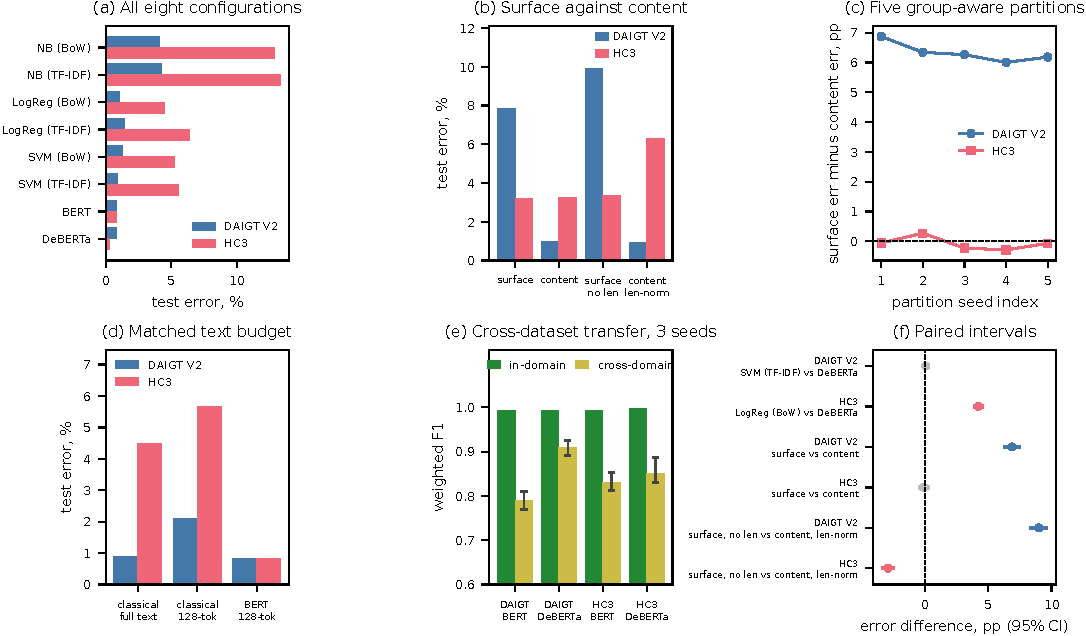
\includegraphics[width=\textwidth]{figures/fig_dashboard.pdf}
\caption{Every headline result in one view. Panels give the model ranking (a), the decomposition with and without the length channel (b), the surface-minus-content difference across five partitions (c), the matched text budget (d), cross-corpus transfer (e), and the paired intervals behind each significance claim (f), where grey marks an interval containing zero.}
\label{fig:dashboard}
\end{figure*}

Figure~\ref{fig:dashboard} collects the results above. Panel (c) is where the central claim stands or falls, with the DAIGT V2 series six to seven points above zero on every partition and the HC3 series straddling it and changing sign. Panel (f) shows the same distinction as intervals, where grey marks those containing zero.